\chapter{Technologies} \label{ch:technologies}

\section{Docker}
When discussing containers, Docker cannot be left out of the discussion. Docker is an open-source platform designed to automate the creation, deployment, scaling and management of containerized applications. It is, by far, the most widely adopted tool for containerization. Docker allows the packaging of applications and their dependencies into lightweight and easily portable containers that can be deployed consistently across a wide range of environments. This portability ensures that applications behave identically, whether running on a developer's laptop, a staging environment, or a production server. To provision containers, Docker uses images. Docker images are read-only templates used to create containers, similar to .iso files for virtual machines, but are more lightweight and versatile. Docker images bundle everything an application needs to run, including the operating system, application code, dependencies, libraries, and configuration metadata. The metadata often includes the entrypoint script, a set of commands executed when the container is instantiated. An important feature of Docker images is their layered architecture. Each layer represents a distinct change, such as adding a file, installing a package, or modifying a configuration. This layered design allows developers to build images on top of existing ones, significantly reducing build times, image sizes, and data transfer requirements. The runtime environment responsible for building, running, and managing containers is the Docker Engine, and it consists of three main components. The first is the Docker Daemon, a background service responsible for managing Docker objects, such as containers, images, volumes, and networks. Next is the Docker Command-Line Interface (CLI), which provides a way to interact with Docker through terminal commands. Finally, the REST API enables programmatic access to Docker's functionalities. Docker images are created using Dockerfiles, which act as blueprints for the image creation process. A Dockerfile contains step-by-step instructions for building an image, including the base image, commands to configure the environment, install dependencies, and metadata such as port configurations and  the entrypoint script. This declarative approach ensures reproducibility, as anyone with the Dockerfile can recreate the same image, ensuring consistency across teams. Since images are meant to be portable and used over multiple environments, remote registries to store and fetch images from are crucial. Docker Hub is a free, widely used registry provided by the wider Docker ecosystem. Hand in hand with containers, Docker enables the creation and management of other resources critical for smooth operation. Volumes are a mechanism for persisting data generated and used by containers. Unlike ephemeral container storage, volumes ensure data remains intact even after container deletion. Docker also creates networks, enabling container interconnectivity, and  communication between containers and the outside world. For handling deployments of multiple containers in a programmatic way, Docker Compose can be utilized. Docker Compose is a tool that utilizes simple YAML files to manage multi-container deployments or applications, by defining services, networks, and volumes required. This approach reduces complexity and enhances reproducibility, making it easier to manage applications with multiple interconnected components. Finally, Docker provides a native container orchestration platform, Docker Swarm, but on a production level it is outclassed by other, more robust and feature-rich solutions, such as bare-metal Kubernetes or cloud Kubernetes services like Amazon Elastic Kubernetes Service (EKS) and Google Kubernetes Engine (GKE) that offer seamless integration and scalability.\cite{containers_docker}


\begin{figure}[!h]
    \graphicspath{ {./diagrams/} }
    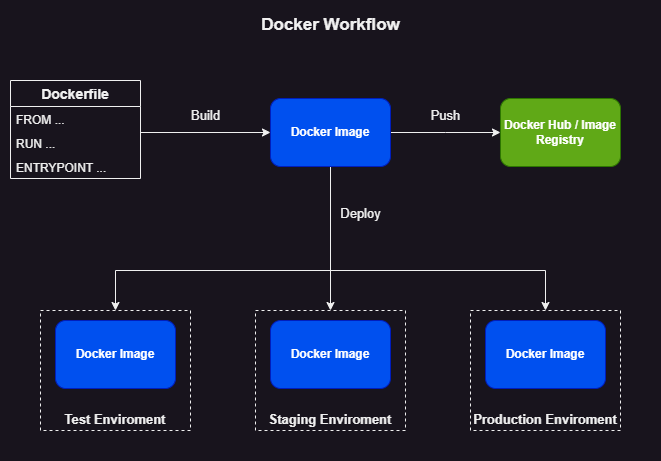
\includegraphics[scale=0.48]{docker_wf.png}
    \centering
    \caption{Docker Workflow}
    \label{fig:docker_wf}
\end{figure}

\section{Prometheus}
Prometheus is an open-source monitoring and alerting toolkit designed to provide flexible, reliable, and robust monitoring for any type of numerical data. Prometheus is considered a foundational tool for observability and a key component of modern monitoring stacks. Prometheus excels in collecting, storing, and querying time-series metrics, making it an ideal choice for monitoring infrastructure, applications, and containerized environments. Prometheus collects and stores metrics as time-series data. Every metric collected is stored alongside a timestamp, which allows tracking and analyzing changes over time. This is invaluable for identifying trends, diagnosing performance bottlenecks, and understanding long-term system behavior. Prometheus operates using a pull-based model, where it periodically scrapes selected targets for metrics. This model ensures efficiency, as Prometheus only fetches the data it needs, and enhances security by not requiring external systems to push data directly into Prometheus. Metrics from various sources are exposed through Exporters, which transform raw data into a Prometheus-readable format. Prometheus includes a large ecosystem of pre-built exporters for common targets such as hardware systems, databases, and cloud platforms. Creating custom exporters is also straightforward, making Prometheus highly adaptable. For retrieving, filtering, and manipulating time-series data collected by Prometheus, Prometheus Query Language (PromQL) can be used. PromQL allows users to extract meaningful insights, create advanced visualizations, and define custom alerting rules. Additionally, Prometheus integrates seamlessly with Alertmanager, a companion tool for managing alerts. Using PromQL expressions, users can define rules to trigger alerts based on specific conditions, such as threshold breaches or anomalies. Alertmanager ensures that alerts are routed to the right channels, such as email, Slack and webhooks. Moreover, For short-lived jobs, which may terminate before Prometheus can scrape their metrics, Prometheus provides the PushGateway. This gateway enables these short-lived jobs to push their metrics to an intermediary location, ensuring no data loss. Prometheus also supports Service Discovery, enabling automatic detection of scrape targets in dynamic environments such as Kubernetes. This eliminates the need for manual configuration, making it ideal for large-scale, constantly changing systems. Prometheus employs a highly optimized, custom-built database for storing time-series data. The database supports fine-grained retention policies, allowing users to define which metrics to retain and for how long, optimizing storage usage. Prometheus edge comes from the ability to label metrics with key-value pairs that provide additional context. This labeling system facilitates easy filtering and aggregation, enabling multidimensional analysis of metrics. Prometheus integrates easily with other tools in the observability ecosystem. While it offers basic visualization capabilities, it is natively compatible with Grafana, the industry-leading visualization platform, enabling users to build interactive and feature-rich dashboards. While Prometheus is optimized for metrics collection, it is not suitable for other types of data, such as logs. To address this, complementary tools, like Loki, are often used alongside Prometheus\cite{Jani2024-mg,Pragathi2024-fa}.

\section{Grafana}
Usually, when utilizing Prometheus to gather metrics, Grafana is employed as the visualization tool of choice. Grafana is an open-source platform for monitoring and observability, designed to enable users to visualize, query, and analyze data from an extensive range of data sources. By transforming raw metrics into actionable insights, Grafana facilitates the creation of complex, interactive dashboards, making it an essential component of most modern monitoring and observability implementations. These dashboards are highly customizable, combining a diverse variety of visualizations, such as line graphs, heatmaps, gauges, tables, and single-stat panels. This flexibility allows teams to represent various types of information, including historical data, real-time system statuses, and long-term trends, in a visually appealing and intuitive manner. Grafana supports integration with a broad array of data sources, including Prometheus, Loki, PostgreSQL, MySQL, and cloud services. Its ability to query multiple sources simultaneously enables advanced, multifaceted analyses, where data from disparate systems can be combined and manipulated for deeper insights. Grafana also has support for variable creation, which allows users to dynamically assign values from the sourced data. This capability enables the construction of dynamic dashboards with parameterized views that adapt to different environments, datasets, or conditions without requiring additional customization. Such dynamic behavior unlocks templating, where reusable dashboards can be developed, significantly enhancing efficiency and consistency across monitoring setups. Grafana excels at centralizing observability, providing a unified view of the health and performance of systems, services, and applications. Its real-time visualizations empower teams to detect and address issues as they emerge, enabling faster response times and minimizing downtime. At the same time, the ability to chart and analyze historical data enables the identification of recurring trends and the prediction of potential problems, thus allowing the implementation of proactive measures to mitigate risks. Lastly, Grafana offers alerting capabilities, same as Prometheus with Alertmanager, that can push notifications on various channels when a set of conditions is met\cite{grafana, promandgraf}.

\begin{figure}[!h]
    \graphicspath{ {./diagrams/} }
    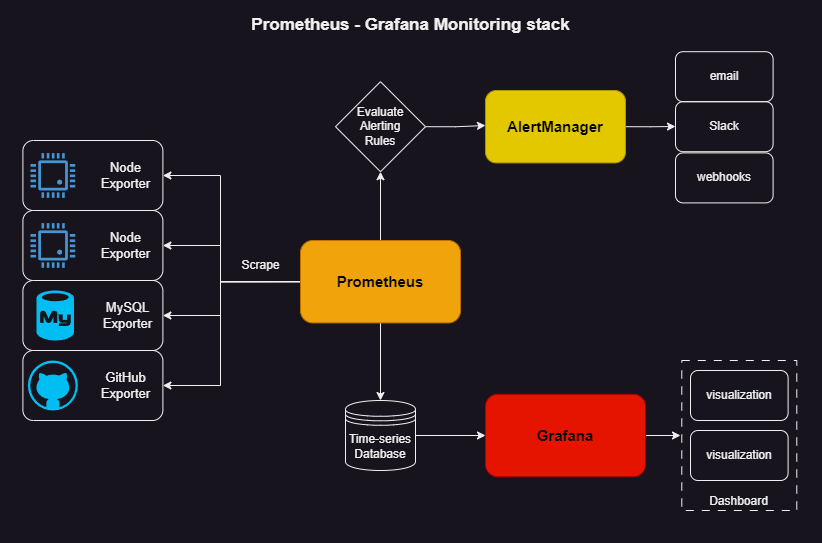
\includegraphics[scale=0.48]{prom-graf.png}
    \centering
    \caption{Prometheus-Grafana Monitoring stack}
    \label{fig:prom_graf}
\end{figure}

\section{MQTT}